\section{Project Management}

\subsection{Milestones}
Several milestones were met in the development of the project, 
the progression through these milestones were used to keep track of the progress 
of the project and to identify areas that needed more attention. 
The progress was projected with a Gantt chart.

The key milestones that were achieved are as follows:
\begin{itemize}
    \item The completion and testing of the back-end API.
    \item The completion and integration of the front-end interface.
    \item The integration of the MPU6050 with the ESP32 and to the back-end API.
    \item Expanding the vision system to locate other colours of beacon.
    \item A communication channel between the FPGA and the ESP32.
    \item Motor driver and control system integration.
    \item The completion of the power delivery system.
\end{itemize}


\subsection{Meetings and Organisation}
Team meetings were held on Microsoft Teams to keep each other up to date. 
In these meetings the progress on each subsystem were discussed 
and then an overall discussion on the integration of the subsystems.

\subsection{Financial Costs}
The majority of costs came from building our chassis. This included the funding for the clear acrylic itself costing £8.07, threaded M10 rods costing £20.14, M10 nuts costing £13.38 and five phototransistors for £2.25. 

Overall, in total we had spent £43.84. All items were carefully evaluated before purchase ensuring that all items were necessary and used. The costs could have been more than halved if we were able to make orders of specific quantities instead of having to order a minimum amount. To prevent waste and encourage growth among our peers, we gifted any spare items we had. 

\begin{figure}
    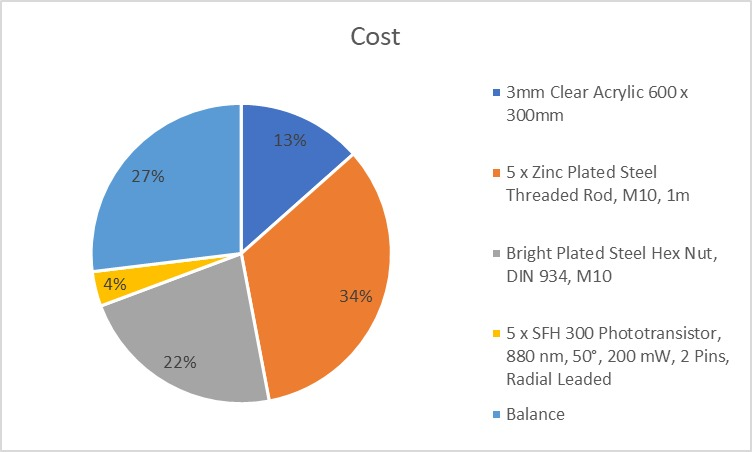
\includegraphics[width=\linewidth]{images/piechart.jpg}
\end{figure}